\documentclass[11pt,a4paper]{article}

\usepackage[utf8]{inputenc}
\usepackage[T1]{fontenc}
\usepackage{lmodern}
\usepackage{amsmath,amssymb,amsfonts}
\usepackage{amsthm}
\usepackage{graphicx}
\usepackage{hyperref}
\usepackage{geometry}
\usepackage[slovene]{babel}      % Slovenian language support
\geometry{a4paper, margin=1in}
\usepackage{titlesec}
\usepackage{enumitem}
\usepackage{caption}
\usepackage{cite}
\usepackage{tikz}
\usepackage{subcaption} % Required for subfigures



% Define the definition environment
\newtheorem{definition}{Definicija}
\newtheorem{lemma}{Lema}
\newtheorem{theorem}{Izrek}
% Define custom environment based on 'proof'
% \newtheorem{proof}{Dokaz}

% Define custom environment for algorithms
\newtheorem{algorithm}{Algoritem}




% % Title formatting
\titleformat{\section}{\large\bfseries}{\thesection.}{0.5em}{}
\titleformat{\subsection}{\normalsize\bfseries}{\thesubsection.}{0.5em}{}

% Metadata
\title{\textbf{Bernsteinovi bazni polinomi treh spremenljivk}}
\author{Nejc Jenko, Petja Murnik}
% \author{Petja Murnik}
\date{\today}

\begin{document}

% Title Page
\maketitle
\break
% \begin{abstract}
% This is the abstract of your article. Write a concise summary of the purpose, methodology, results, and conclusions here.
% \end{abstract}

\section{Uvod}

Pri predavanjih predmeta RPGO smo se ukvarjali z Bernsteinovimi baznimi polinomi ene in dveh 
spremenljivk, ki se pogosto uporabljajo pri različnih aplikacijah
v numerični matematiki. Njihova preprosta definicija in koristne lastnosti,
kot sta pozitivnost in lastnost particije enote, jih postavljajo v ospredje pri reševanju problemov
kot so aproksimacija funkcij, interpolacija ter modeliranje geometrijskih objektov.

V tej nalogi bomo raziskali razširitev
Bernsteinovih baznih polinomov na tri spremenljivke.
Ta posplošitev omogoča uporabo teh polinomov v še bolj zahtevnih aplikacijah,
kot so modeliranje tridimenzionalnih površin in simulacija geometrijskih oblik.
Poleg tega bomo podrobneje obravnavali njihove matematične lastnosti ter predstavili nekaj praktičnih primerov 
uporabe v računalniški grafiki in drugih področjih.


\section{Prostor polinomov treh spremenljivk} 

\begin{definition}\label{def_prostor}
    Naj bo $d \in \mathbb{N}_0$. \textbf{Prostor polinomov treh spremenljivk} stopnje $d$ je definiran kot
    \begin{equation}
        \mathcal{P}_d = \left\{ p : p(x, y, z) = \sum_{0 \leq i + j + k \leq d} a_{ijk} x^i y^j z^k , \ a_{ijk} \in \mathbb{R} \right\}    \end{equation}
\end{definition}

\begin{lemma}
    Naj bo $\mathcal{P}_d$ definiran kot v definiciji \ref{def_prostor}.
    Potem velja, da je $\dim \mathcal{P}_d = \binom{d+3}{3} $. 
    Nadalje monomi $\left\{x^i y^j z^k \right\}_{0 \le i  + j + k \le d}$ tvorijo njegovo bazo.
\end{lemma}

Preden se lotimo dokaza leme, vpeljimo noticajo odvodov, 
ki nam bo prišla prav tako pri dokazu kot tudi 
v nadaljevanju. Naj bo $\text{D}^l_w$ operator parcialniega odvoda po
spremenljivki $w$ reda $l$. Potem definiramo 
$\text{D}^\alpha := \text{D}^{\alpha_1}_x \text{D}^{\alpha_2}_y \text{D}^{\alpha_3}_z$
za $\alpha = \left(\alpha_1 , \alpha_2 , \alpha_3 \right)$,
kjer je $\alpha_1,\alpha_2, \alpha_3 \in \mathbb{N}_0$ 
ter vpeljimo še $|\alpha| := \alpha_1 + \alpha_2 + \alpha_3$.

\begin{proof}
    Opazimo najprej, da monomi oblike $\{x^i y^j z^k\}_{0 \le i  + j + k \le d}$
    razpenjanjo $\mathcal{P}_d$, kar sledi direktno it definicije 
    prostora. Opazimo tudi, da 
    $|\left(i, j , k\right): 0\le i+j+k \le d , i,j,k \in \mathbb{N}_0| = \binom{d+3}{3} = \dim\mathcal{P}_d$.
    Pokazati moramo še linearno neodvisnost.  

    Predpostavimo, da je polinom $p(x,y,z) =\sum_{0 \le i  + j + k \le d} a_{ijk} x^i y^j z^k $
    identično enak 0. Potem so tudi vsi njegovi mešani odvodi identično enaki 0.
    Po drugi strani pa z direktnim odvajanjem dobimo
    $D^i_xD^j_yD^z_k p(x,y,z)|_{x =0 ,y =0, z = 0} = a_{ijk}$ za vsak 
    $0 \le i  + j + k \le d$. Torej linearna neodvisnost velja, ter
    je s tem dokazana lema.
\end{proof}

V nadaljevanju bomo prestavili drugo bazo prostora $\mathcal{P}_d$, zato 
nadaljne lastnosti baze monomov ne bomo raziskovali. Za uvedbo Bernsteinovih
baznih polinomov, potrebujemo uvedbo baricentričnih koordinat glede na 
tetraeder, kar je vpeljano v naslednjem razdelku.

Pred tem pa pa prestavimo še lemo, ki nam pove, kako oceniti 
normo polinoma $p \in \mathcal{P}_n$.

\begin{lemma}\label{lema_norma}
    Naj bo $T$ tetraeder z volumnom $V_T$, potem obstaja 
    konstanta $K$ odvisna le od $d$, da za vsak  $p \in \mathcal{P}_d$ ter $1 \le q < \infty$
    \begin{equation}
        V_T^{-1/q} \left\lVert p \right\rVert_{q,T} \le  \left\lVert p \right\rVert_{\infty l, T} \le K V_T^{-1/q} \left\lVert p \right\rVert_{q,T},
    \end{equation}
    kjer je $\left\lVert \cdot{} \right\rVert_{q,T}$ standardna $L_q$ norma 
    glede na tetraeder $T$.
\end{lemma}

\begin{proof}
    Za prvo neenakost računamo
    \begin{equation*}
        \int_{T} |p(t)|^q dt \le 
        \int_{T} \left( \sup_{t \in T} |p(t)| \right) ^q dt
        = \left( \sup_{t \in T} |p(t)| \right)^q \int_{T}1dt
        = \left\lVert p \right\rVert_{\infty , T}^{q} \cdot V_T
    \end{equation*}
    ter če začetek in konec $q$-korenimo, dobimo željeno.

    Za drugo neenakost pa uporabimo dejstvo, da je $\mathcal{P}_d$ končno dimenzionalen prostor, zato so vse norme ekvivalentne. Torej obstaja konstanta $K$, odvisna le od $d$, da velja
    \begin{equation*}
        \left\lVert p \right\rVert_{\infty, T} \leq K \left\lVert p \right\rVert_{q,T}.
    \end{equation*}
    Združimo obe neenakosti in dobimo
    \begin{equation*}
        V_T^{-1/q} \left\lVert p \right\rVert_{q,T} \leq  \left\lVert p \right\rVert_{\infty, T} \leq K V_T^{-1/q} \left\lVert p \right\rVert_{q,T}.
    \end{equation*}
    S tem je lema dokazana.
\end{proof}

%pomoje bzv
% \begin{theorem}
%     TODO
% \end{theorem}

\section{Baricentrične koordinate}

Analogno z ravninskim primerom, želimo tudi 
v $\mathbb{R}^3$ uvesti stabilnejšo bazo za prostor 
$\mathcal{P}_d$, ki bo temeljila na Bernsteinovih baznih polinomih,
za kar moramo najeprej vpeljati baricentrične koordinate glede na
tetraeder.

\begin{definition}
    Rečemo, da je tetraeder $T = \langle V_1, V_2, V_3, V_4 \rangle$ \textbf{nedegeneriran}, če ima neničelen volumen. Rečemo, da so vozlišča $V_1 , V_2 , V_3, V_4$ tetraedra $T$ v \textbf{kanoničnem redu}, če lahko $T$ rotiramo in transliramo  tako, da ploskev $\langle V_1, V_2, V_3\rangle$ leži v ravnini $z = 0$ in je pozitivno orientirana ter je $z$ koordinata vozlišča $V_4$ pozitivna.
\end{definition}

Od sedaj naprej predpostavimo, da je tetraeder $T = \langle V_1, V_2, V_3,V_4 \rangle$ v kanoničnem redu in ni degeneriran. 
Za vozlišče $V_i$ velja $V_i = (x_i, y_i, z_i)$. Postavimo 

\begin{align}
    M := \begin{bmatrix}
        1 & 1 & 1 & 1 \\
        x_1 & x_2 & x_3 & x_4 \\
        y_1 & y_2 & y_3 & y_4 \\
        z_1 & z_2 & z_3 & z_4
    \end{bmatrix}.
\end{align}
Znano je dejstvo, da velja $\text{det}(M) = 6V_T$, kjer je $V_T$ volumen tetraedra $T$. 


\begin{lemma}\label{lema_baricentricne}
    Naj bo $T = \langle V_1, V_2, V_3, V_4 \rangle$ tetraeder v kanoničnem redu.
    Potem za vsako točko $V = (x,y,z) \in \mathbb{R}^3$ obstajajo enolično določene
     $\phi_1, \phi_2, \phi_3, \phi_4 \in \mathbb{R}$,
    da velja 
    \begin{equation}\label{eq_baricentricne}
        V = \phi_1 V_1 + \phi_2 V_2 + \phi_3 V_3 + \phi_4 V_4
    \end{equation} ter 
    \begin{equation}\label{eq_particija}
        \phi_1 + \phi_2 + \phi_3 + \phi_4 = 1 .
    \end{equation}
    Vrednostim $\phi_1, \phi_2, \phi_3, \phi_4$ rečemo \textbf{baricentrične 
    koordinate} točke $V$ glede na tetraeder $T$.
\end{lemma}

\begin{proof}
    Enačbi \ref{eq_baricentricne} in \ref{eq_particija} sta ekvivalentni
    sledečemu nesingularnem sistemu:
    \begin{align}
        M \begin{bmatrix}\phi_1 \\ \phi_2 \\ \phi_3 \\ \phi_4 \end{bmatrix} = \begin{bmatrix}
            1 \\ x \\ y \\ z \end{bmatrix}.
    \end{align}
\end{proof}

V dokazu opazimo, da z uporabo Cramerjevega pravila dobimo
\begin{align}\label{eq_cramer}
    \phi_1 = \frac{1}{\text{det}(M)}
    \begin{vmatrix}
        1 & 1 & 1 & 1 \\
        x & x_2 & x_3 & x_4 \\
        y & y_2 & y_3 & y_4 \\
        z & z_2 & z_3 & z_4
    \end{vmatrix}.
\end{align}
Podobno bi dobili za $\phi_2, \phi_3, \phi_4$. 
Opazimo tudi, da lahko $i$-to baricentrično koordinato izračunamo
kot $\frac{V_{\widetilde{T_i}}}{V_T}$, kjer je $V_{\widetilde{T_i}}$
prostornina tetraedra, ki ga dobimo, če zamenjamo $i$-to vozlišče
s točko $V$. 
Naprej bi z razvojem determinante v izrazu \eqref{eq_cramer}
dokazali naslednjo lemo.

\begin{lemma}
    Za vsak $i = 1, 2, 3, 4$ je funkcija $\phi_i$ linearni polinom
    v $x, y, z$, ki doseže vrednost $1$ v oglišču $V_i$ in
    izgine v vseh točkah na ploskvi tetraedra $T$, ki leži
    nasproti $V_i$. Poleg tega velja
    $0 \leq \phi_i \leq 1$, kadar $(x, y, z)$ leži v $T$.
\end{lemma}

\section{Bernsteinovi bazni polinomi}

\begin{definition}
    Naj bo $T = \langle V_1, V_2, V_3, V_4 \rangle$ tetraeder v kanoničnem redu.
    \textbf{Bernsteinov bazni polinom} stopnje $n$ glede na tetraeder $T$ je definiran kot
    \begin{equation}
        B_{ijkl}^d := \frac{d!}{i!j!k!l!} \phi_1^i \phi_2^j \phi_3^k \phi_4^l, \quad i + j + k + l = d,
    \end{equation}
    kjer je $\phi_1, \phi_2, \phi_3, \phi_4$ baricentrične koordinate funkcije
    glede na tetraeder $T$. V primeru, ko je kateri izmed indeksov $i, j, k, l$ negativen, 
    nastavimo $B_{ijkl}^d = 0$.
\end{definition}

\begin{theorem}\label{izrek_bernstein}
    Bernsteinovi bazni polinomi $B_{ijkl}^d$ tvorijo bazo prostora $\mathcal{P}_d$.
    Prav tako velja 
    \begin{equation}\label{eq_partcija_enote}
        \sum_{i+j+k+l = d} B_{ijkl}^d(V) = 1, \quad \forall V \in \mathbb{R}^3     
    \end{equation}
    ter
    \begin{equation}
        0 \leq B_{ijkl}^d(V) \leq 1, \quad \forall V \in T.
    \end{equation}
\end{theorem}

\begin{proof}
    Označimo z $\mathcal{B}_d := \left\{ B_{ijkl}^d  \right\}_{0\leq i+j+k+l \leq 1}$ množica
    Bernsteinovih polinomov. 

    Za dokaz enakosti \eqref{eq_partcija_enote} pokažemo, da velja $$1 = \left( \phi_1 + \phi_2 + 
    \phi_3 + \phi_4  \right)^d = \sum_{i+j+k+l = d} \frac{d!}{i!j!k!l!} 
    \phi_1^i \phi_2^j \phi_3^k \phi_4^l$$.

    Tu opazimo tudi, da je v $1 \in \text{Lin} \mathcal{B}_d$. Dokaza izjave
    o bazi prostora, se bomo lotili z induklcijo po $d$. Za $d = 0$ smo pokazali zgoraj. Lotimo
    se sedaj primera, ko je $d = 1$.

    Če enačbo \eqref{eq_baricentricne} zapišemo kot 
    \begin{equation*}
        \begin{bmatrix}
            x \\ y \\ z 
        \end{bmatrix} = 
        \phi_1\begin{bmatrix} x_1 \\ y_1 \\ z_1\end{bmatrix} +
        \phi_2\begin{bmatrix} x_2 \\ y_2 \\ z_2\end{bmatrix} +  
        \phi_3\begin{bmatrix} x_3 \\ y_3 \\ z_3\end{bmatrix} +
        \phi_4\begin{bmatrix} x_4 \\ y_4 \\ z_4\end{bmatrix}
    \end{equation*}
    ter pogledamo le prvo vrstico in upoštevamo $1 = \sum_{i+j+k+l}B_{ijkl}^{d-1}$ računamo
    $$x = \left(x_1 \phi_1 + x_2 \phi_2 + x_3 \phi_3 +x_4 \phi_4 \right)  \sum_{i+j+k+l = d-1} B_{ijkl}^{d-1} = \star $$
    Poglejmo posebej prvi člen
    \begin{align*}
        x_1 \phi_1 &= x_1 \phi_1 \sum_{i+j+k+l = d-1} B_{ijkl}^{d-1} =  
            x_1  \sum_{i+j+k+l = d-1} \frac{(d-1)!}{i!j!k!l!} \phi_1^{i+1} \phi_2^j \phi_3^k \phi_4^l 
            \\ & = \sum_{i = 0}^{d-1} \left(\sum_{j+k+l = d-1-i} x_1 \frac{(d-1)!}{i!j!k!l!} \phi_1^{i+1} \phi_2^j \phi_3^k \phi_4^l \right) = 
            \\ & = \sum_{\tilde{\imath} = 1}^{d} \left(  \sum_{j+k+l = d-\tilde{\imath}} \frac{x_i \tilde{\imath}}{d} \frac{d!}{\tilde{\imath}! j!k!l!}     \phi_1^{\tilde{\imath}} \phi_2^j \phi_3^k \phi_4^l  \right) = 
            \\ & = \sum_{\tilde{\imath} = 0}^{d} \left( \sum_{j+k+l = d- \tilde{\imath}} \frac{\tilde{\imath} x_1}{d} B_{\tilde{\imath}jkl}^d\right) = 
            \sum_{i+j+k+l = d} \frac{i}{d} x_1 B_{ijkl}^d,
    \end{align*}
    kjer smo v prehodu na 3. vrstico označili $\tilde{\imath} = i+1$. Združimo vse člene ter 
    dobimo 
    \begin{align*}
         \star
        = \sum_{i+j+k+l = d} \frac{ix_1 + jx_2 + k x_3 +l x_4}{d} B_{ijkl}^d(x,y,z)
    \end{align*}
    Podobna izraza bi dobili 
    za spremenljivki $y$ in $z$, s čimer smo torej pokazali, 
    da izjava velja za $d = 1$ ( saj ulomek tolmačimo kot konsanto 
    ter je to ravno definicija linearne ogrinjače). Lotimo se sedaj indukcijskega koraka. 

    Naj trditev velja za vse polinome oblike $x^\mu y^\nu z^\kappa$, 
    kjer $\mu + \nu + \kappa \leq  d-1$. Potem za $\mu + \nu + \kappa =  d$ ter 
    nek $c_{ijkl}$ velja  
    \begin{align*}
        x^\mu y^\nu z^\kappa &= x \left(x^{\mu-1} y^\nu z^\kappa\right) = 
        \left(x_1 \phi_1 + x_2 \phi_2 + x_3 \phi_3 +x_4 \phi_4 \right) \sum_{i+j+k+l = d-1}c_{ijkl} B_{ijkl}^{d-1}(x,y,z) =
        \\ & =  x \sum_{i+j+k+l = d}d_{ijkl} B_{ijkl}^{d}(x,y,z)
        ,
    \end{align*}
    kjer je $d_{ijkl}$ dobljen na podoben način kot v primeru $d = 1$. Skupaj z dejstvom, 
    da je $\text{dim}\left(\mathcal{P}_d \right)=  \binom{d+3}{3}$ enako številu baznih funkcij 
    v $\mathcal{B}_d$ dokažemo izjavo, da Bernsteinovi bazni polinomi tvorijo 
    bazo $\mathcal{P}_d$. 

    Izjava o spodnji ter zgornji meji Bernsteinovih baznih funkcij sledi direktno iz
    lastnosti baricentričnih koordinat.
\end{proof}

Iz izreka \ref{izrek_bernstein} sledi, da lahko vsak polinom $p \in \mathcal{P}_d$
lahko zapišemo na enoličen način kot
\begin{equation}\label{eq_Bforma}
    p = \sum_{i+j+k+l = d} c_{ijkl} B_{ijkl}^d.
\end{equation}
Tak zapis imenujemo \textbf{B-forma} ter koeficente $c_{ijkl}$ \textbf{B-koeficienti}.
Množico domenskih točk definiramo ter označimo kot
\begin{equation}
    \mathcal{D}_{d,T} := 
    \left\{
        \zeta_{ijkl}^T:= \frac{i V_1 + j V_2 + k V_3 + l V_4}{d}
     \right\}_{i + j+ k+l = d}.
\end{equation}

%%% SLIKE

\begin{figure}[h]
    \centering
    % ---- Subfigure d = 2 (blue) ----
    \begin{subfigure}[b]{0.45\linewidth}
        \centering
        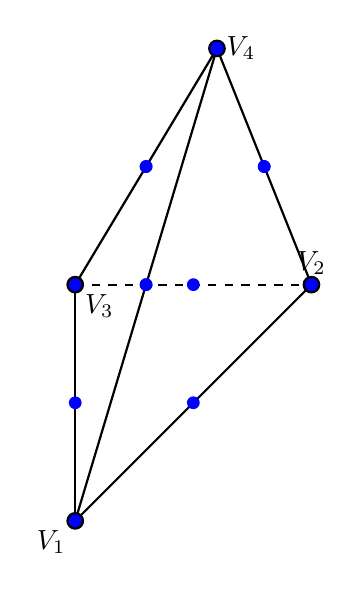
\begin{tikzpicture}[scale=3, z={(0.6cm,2cm)}] 
            \coordinate (V_1) at (0, 0, 0);
            \coordinate (V_2) at (0,1, 0);
            \coordinate (V_3) at (1,1,0);
            \coordinate (V_4) at (0,0,1);
        
            % Draw edges
            \draw[thick] (V_1) -- (V_2);
            \draw[thick,dashed] (V_2) -- (V_3);
            \draw[thick] (V_1) -- (V_4);
            \draw[thick] (V_2) -- (V_4);
            \draw[thick] (V_3) -- (V_4);
            \draw[thick] (V_3) -- (V_1);
        
            % Add vertice
            \filldraw[black] (V_1) circle (1pt) node[below left] {$V_1$};
            \filldraw[black] (V_2) circle (1pt) node[below right] {$V_3$};
            \filldraw[black] (V_3) circle (1pt) node[above] {$V_2$};
            \filldraw[black] (V_4) circle (1pt) node[right] {$V_4$};
        
            \coordinate (V_0_0_2) at (0.0, 0.0, 1.0);
            \filldraw[blue,] (V_0_0_2) circle (0.7pt);
            \coordinate (V_0_0_2) at (0.0, 0.0, 1.0);
            \filldraw[blue,] (V_0_0_2) circle (0.7pt);
            \coordinate (V_0_0_2) at (0.0, 0.0, 1.0);
            \filldraw[blue,] (V_0_0_2) circle (0.7pt);
            \coordinate (V_0_0_1) at (0.5, 0.5, 0.5);
            \filldraw[blue,] (V_0_0_1) circle (0.7pt);
            \coordinate (V_0_0_1) at (0.5, 0.5, 0.5);
            \filldraw[blue,] (V_0_0_1) circle (0.7pt);
            \coordinate (V_0_0_0) at (1.0, 1.0, 0.0);
            \filldraw[blue,] (V_0_0_0) circle (0.7pt);
            \coordinate (V_0_1_1) at (0.0, 0.5, 0.5);
            \filldraw[blue,] (V_0_1_1) circle (0.7pt);
            \coordinate (V_0_1_1) at (0.0, 0.5, 0.5);
            \filldraw[blue,] (V_0_1_1) circle (0.7pt);
            \coordinate (V_0_1_0) at (0.5, 1.0, 0.0);
            \filldraw[blue,] (V_0_1_0) circle (0.7pt);
            \coordinate (V_0_2_0) at (0.0, 1.0, 0.0);
            \filldraw[blue,] (V_0_2_0) circle (0.7pt);
            \coordinate (V_1_0_1) at (0.0, 0.0, 0.5);
            \filldraw[blue,] (V_1_0_1) circle (0.7pt);
            \coordinate (V_1_0_1) at (0.0, 0.0, 0.5);
            \filldraw[blue,] (V_1_0_1) circle (0.7pt);
            \coordinate (V_1_0_0) at (0.5, 0.5, 0.0);
            \filldraw[blue,] (V_1_0_0) circle (0.7pt);
            \coordinate (V_1_1_0) at (0.0, 0.5, 0.0);
            \filldraw[blue,] (V_1_1_0) circle (0.7pt);
            \coordinate (V_2_0_0) at (0.0, 0.0, 0.0);
            \filldraw[blue,] (V_2_0_0) circle (0.7pt);
        \end{tikzpicture}
    \end{subfigure}
    \begin{subfigure}[b]{0.45\linewidth}
        \centering
        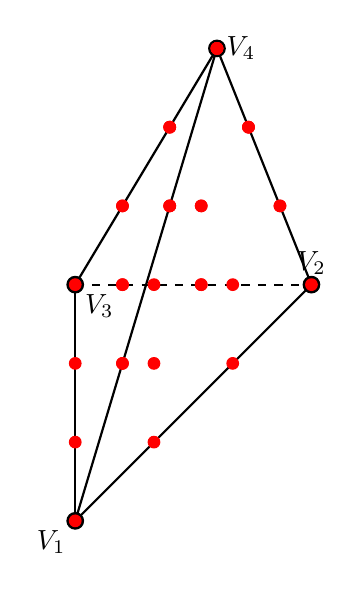
\begin{tikzpicture}[scale=3, z={(0.6cm,2cm)}] 
            % Define vertices of the tetrahedron
            \coordinate (V_1) at (0, 0, 0);
            \coordinate (V_2) at (0,1, 0);
            \coordinate (V_3) at (1,1,0);
            \coordinate (V_4) at (0,0,1);

            % Draw edges
            \draw[thick] (V_1) -- (V_2);
            \draw[thick,dashed] (V_2) -- (V_3);
            \draw[thick] (V_1) -- (V_4);
            \draw[thick] (V_2) -- (V_4);
            \draw[thick] (V_3) -- (V_4);
            \draw[thick] (V_3) -- (V_1);

            % Add vertice
            \filldraw[black] (V_1) circle (1pt) node[below left] {$V_1$};
            \filldraw[black] (V_2) circle (1pt) node[below right] {$V_3$};
            \filldraw[black] (V_3) circle (1pt) node[above] {$V_2$};
            \filldraw[black] (V_4) circle (1pt) node[right] {$V_4$};


            \coordinate (V_0_0_3) at (0.0, 0.0, 1.0);
            \filldraw[red,] (V_0_0_3) circle (0.7pt);
            \coordinate (V_0_0_3) at (0.0, 0.0, 1.0);
            \filldraw[red,] (V_0_0_3) circle (0.7pt);
            \coordinate (V_0_0_3) at (0.0, 0.0, 1.0);
            \filldraw[red,] (V_0_0_3) circle (0.7pt);
            \coordinate (V_0_0_3) at (0.0, 0.0, 1.0);
            \filldraw[red,] (V_0_0_3) circle (0.7pt);
            \coordinate (V_0_0_2) at (0.3333333333333333, 0.3333333333333333, 0.6666666666666666);
            \filldraw[red,] (V_0_0_2) circle (0.7pt);
            \coordinate (V_0_0_2) at (0.3333333333333333, 0.3333333333333333, 0.6666666666666666);
            \filldraw[red,] (V_0_0_2) circle (0.7pt);
            \coordinate (V_0_0_2) at (0.3333333333333333, 0.3333333333333333, 0.6666666666666666);
            \filldraw[red,] (V_0_0_2) circle (0.7pt);
            \coordinate (V_0_0_1) at (0.6666666666666666, 0.6666666666666666, 0.3333333333333333);
            \filldraw[red,] (V_0_0_1) circle (0.7pt);
            \coordinate (V_0_0_1) at (0.6666666666666666, 0.6666666666666666, 0.3333333333333333);
            \filldraw[red,] (V_0_0_1) circle (0.7pt);
            \coordinate (V_0_0_0) at (1.0, 1.0, 0.0);
            \filldraw[red,] (V_0_0_0) circle (0.7pt);
            \coordinate (V_0_1_2) at (0.0, 0.3333333333333333, 0.6666666666666666);
            \filldraw[red,] (V_0_1_2) circle (0.7pt);
            \coordinate (V_0_1_2) at (0.0, 0.3333333333333333, 0.6666666666666666);
            \filldraw[red,] (V_0_1_2) circle (0.7pt);
            \coordinate (V_0_1_2) at (0.0, 0.3333333333333333, 0.6666666666666666);
            \filldraw[red,] (V_0_1_2) circle (0.7pt);
            \coordinate (V_0_1_1) at (0.3333333333333333, 0.6666666666666666, 0.3333333333333333);
            \filldraw[red,] (V_0_1_1) circle (0.7pt);
            \coordinate (V_0_1_1) at (0.3333333333333333, 0.6666666666666666, 0.3333333333333333);
            \filldraw[red,] (V_0_1_1) circle (0.7pt);
            \coordinate (V_0_1_0) at (0.6666666666666666, 1.0, 0.0);
            \filldraw[red,] (V_0_1_0) circle (0.7pt);
            \coordinate (V_0_2_1) at (0.0, 0.6666666666666666, 0.3333333333333333);
            \filldraw[red,] (V_0_2_1) circle (0.7pt);
            \coordinate (V_0_2_1) at (0.0, 0.6666666666666666, 0.3333333333333333);
            \filldraw[red,] (V_0_2_1) circle (0.7pt);
            \coordinate (V_0_2_0) at (0.3333333333333333, 1.0, 0.0);
            \filldraw[red,] (V_0_2_0) circle (0.7pt);
            \coordinate (V_0_3_0) at (0.0, 1.0, 0.0);
            \filldraw[red,] (V_0_3_0) circle (0.7pt);
            \coordinate (V_1_0_2) at (0.0, 0.0, 0.6666666666666666);
            \filldraw[red,] (V_1_0_2) circle (0.7pt);
            \coordinate (V_1_0_2) at (0.0, 0.0, 0.6666666666666666);
            \filldraw[red,] (V_1_0_2) circle (0.7pt);
            \coordinate (V_1_0_2) at (0.0, 0.0, 0.6666666666666666);
            \filldraw[red,] (V_1_0_2) circle (0.7pt);
            \coordinate (V_1_0_1) at (0.3333333333333333, 0.3333333333333333, 0.3333333333333333);
            \filldraw[red,] (V_1_0_1) circle (0.7pt);
            \coordinate (V_1_0_1) at (0.3333333333333333, 0.3333333333333333, 0.3333333333333333);
            \filldraw[red,] (V_1_0_1) circle (0.7pt);
            \coordinate (V_1_0_0) at (0.6666666666666666, 0.6666666666666666, 0.0);
            \filldraw[red,] (V_1_0_0) circle (0.7pt);
            \coordinate (V_1_1_1) at (0.0, 0.3333333333333333, 0.3333333333333333);
            \filldraw[red,] (V_1_1_1) circle (0.7pt);
            \coordinate (V_1_1_1) at (0.0, 0.3333333333333333, 0.3333333333333333);
            \filldraw[red,] (V_1_1_1) circle (0.7pt);
            \coordinate (V_1_1_0) at (0.3333333333333333, 0.6666666666666666, 0.0);
            \filldraw[red,] (V_1_1_0) circle (0.7pt);
            \coordinate (V_1_2_0) at (0.0, 0.6666666666666666, 0.0);
            \filldraw[red,] (V_1_2_0) circle (0.7pt);
            \coordinate (V_2_0_1) at (0.0, 0.0, 0.3333333333333333);
            \filldraw[red,] (V_2_0_1) circle (0.7pt);
            \coordinate (V_2_0_1) at (0.0, 0.0, 0.3333333333333333);
            \filldraw[red,] (V_2_0_1) circle (0.7pt);
            \coordinate (V_2_0_0) at (0.3333333333333333, 0.3333333333333333, 0.0);
            \filldraw[red,] (V_2_0_0) circle (0.7pt);
            \coordinate (V_2_1_0) at (0.0, 0.3333333333333333, 0.0);
            \filldraw[red,] (V_2_1_0) circle (0.7pt);
            \coordinate (V_3_0_0) at (0.0, 0.0, 0.0);
            \filldraw[red,] (V_3_0_0) circle (0.7pt);
        \end{tikzpicture}
        % \caption{Tetraeder s pripadajočimi domenskimi točkami stopnje \( d = 3 \).}
        % \label{fig:tetrahedron}  
    \end{subfigure}
    % ---- Common Caption ----
\caption{Domenske točke tetraedra stopnje \( d = 2 \) (modre) in \( d = 3 \) (rdeče).}
\label{fig:tetrahedron}
\end{figure}







Nadalje pripišemo vsaki domenski točki $\zeta_{ijkl}^T$ B-koeficent
$c_{ijkl}$ za $i +j+k+l = d$. Torej lahko zapišemo B-koeficente kot $\left\{
    c_{\zeta}
\right\}_{\zeta \in \mathcal{D}_{d,T}}$ tako da če $\zeta = \zeta_{ijkl}^T$,
potem je $c_{\zeta} = c_{ijkl}$.

\begin{theorem}
    Naj bo $p \in \mathcal{P}_d$ zapisan v obliki B-forme \eqref{eq_Bforma}. Označimo 
    z $\text{F}_1 := \langle V_2,V_3,V_4 \rangle$ ploskev tetraedra $T$ nasproti vozlišču $V_1$.
    Potem velja 
    \begin{equation*}
        p|_{\text{F}_1} = \sum_{j+k+l = d} c_{0jkl}B_{0jkl}^d = 
            \sum_{j+k+l}c_{jkl}^{\text{F}_1} B_{jkl}^{\text{F}_1,d},
    \end{equation*}
    kjer $c_{jkl}^{\text{F}_1}:=c_{0jkl}$ ter so $B_{jkl}^{\text{F}_1,d}$
    Bernsteinovi bazni polinomi stopnje $d$ glede na trikotnik $\text{F}_1$ .
\end{theorem}

Podobne formule veljajo za ostale ploskve tetraedra $T$.

\begin{proof}
    Upoštevaje dejstvo, da je $B_{0jkl}^d = 0$ za vsako $V \in \text{F}_1$ (ker je 
    tam $\phi_1 = 0$), trditev sledi nemudoma.
\end{proof}

Brez dokaza, ki bi med drugimi zahtevnejšimi izreki, uporabil 
tudi lemo \ref{lema_norma},
podajmo še spodnjo trditev od stabilnosti B-forme.
\begin{theorem}
    Naj bo $T$ tetraeder, katerega volumen je $V_T$. Potem za vsak
    polinom $p$ zapisan v obliki B-forme \eqref{eq_Bforma} ter za $1 \leq q \leq \infty$
    velja neenakost
    \[
    \frac{V_T^{1/q}}{K} \| c \|_q \leq \| p \|_{q,T} \leq V_T^{1/q} K \| c \|_q,
    \]
    kjer je $K$ konstanta, ki je odvisna samo od $d$.
\end{theorem}

\section{de Castljaujev algoritem}

V tem razdelku bomo predstavili de Casteljaujev algoritem. Algoritem omogoča učinkovito in stabilno izračunavanje vrednosti polinomov v B-formi. Algoritem temelji na rekurzivni zvezi:

\begin{align*}
 B_{ijkl}^d = \phi_1 B_{i-1,j,k,l}^{d-1} + \phi_2 B_{i,j-1,k,l}^{d-1} + \phi_3 B_{i,j,k-1,l}^{d-1} + \phi_4 B_{i,j,k,l-1}^{d-1}, 
\end{align*}

\begin{theorem}
    Naj bo $p \in \mathcal{P}_d$ zapisan v obliki B-forme \eqref{eq_Bforma}. Njegove koeficiente označimo z $c_{ijkl}^{(0)} = c_{ijkl}, i+j+l+k = d$.
    Naj ima točka $V$ baricentrične koordinate $\phi_1, \phi_2, \phi_3, \phi_4$.

    Potem velja:
    $$
    p(V) = \sum_{i+j+k+l = d} c_{ijkl}^{(d)} B_{ijkl}^d(V),
    $$

    kjer so  $c_{ijkl}^{(r)}$ definirani kot:
    \begin{align*}
        c_{ijkl}^{(r)} = \phi_1 c_{i-1,j,k,l}^{(r-1)} + \phi_2 c_{i,j-1,k,l}^{(r-1)} + \phi_3 c_{i,j,k-1,l}^{(r-1)} + \phi_4 c_{i,j,k,l-1}^{(r-1)},
    \end{align*}
    za i+j+k+l = d, r = 1, 2, \ldots, d.
\end{theorem}

Direktno iz tega izreka sledi želeni algoritem.

\begin{algorithm}{(de Casteljaujev algoritem)}
    \begin{enumerate}
        \item Za $r = 0$ nastavi $c_{ijkl}^{(0)} = c_{ijkl}$ za $i+j+k+l = d$.
        \item Za $r = 1, 2, \ldots, d$ izračunaj
        \begin{align*}
            c_{ijkl}^{(r)} = \phi_1 c_{i-1,j,k,l}^{(r-1)} + \phi_2 c_{i,j-1,k,l}^{(r-1)} + \phi_3 c_{i,j,k-1,l}^{(r-1)} + \phi_4 c_{i,j,k,l-1}^{(r-1)},
        \end{align*}
        za $i+j+k+l = d$.
        \item Vrednost polinoma $p$ v točki $V$ je enaka
        \begin{align*}
            p(V) = \sum_{i+j+k+l = d} c_{ijkl}^{(d)} B_{ijkl}^d(V).
        \end{align*}
    \end{enumerate}
\end{algorithm}

\section{Zaključek}



\begin{thebibliography}{99}

    \bibitem{LaiSchumaker} 
    M. J. Lai, L. Schumaker, \textit{Spline Functions on Triangulations}, 
    Cambridge University Press, 2007, strani 434–443.

    \bibitem{Farin} 
    G. Farin, \textit{Curves and Surfaces for CAGD: A Practical Guide}, 
    Elsevier, 2001.

\end{thebibliography}


\end{document}

